% \section{Цель работы}
% \begin{frame}[plain]
%     \frametitle{Цель работы}
%         Исследование и совершенствование методов оптимизации для задач большой размерностью, не обладающих достаточной гладкостью для применения классических методов. Предприняты шаги по расширению доступного класса задач, рассматриваются аналоги условия Липшица, которые позволяют сохранить свойственную липшицевым задачам оптимальные оценки скорости сходимости.
% \end{frame}

\begin{frame}{[1] Введение. Определения и оценки.}
    Липшицевость:
    $$
    |f(y) - f(x)| \leq M \norm{y-x}_2 \;\;\; \forall x, y \in Q
    $$

    Гладкость (условие Липшица градиента):
    $$
    \norm{\nabla f(x) - \nabla f(y)}_2 \leq L \norm{x - y}_2 \;\;\; \forall x, y \in Q
    $$
    
    \begin{table}[h]
        \centering
        \begin{tabular}{|c|c|c|}
            \hline
             & \makecell{$|f(y) - f(x)| \leq$ \\ $\leq M \| y - x \|_2$} & \makecell{$\|\nabla f(y) - \nabla f(x)\|_2 \leq $\\ $\leq L \| y - x \|_2$} \\
            \hline
            $f(x)$ -- выпукла & $\mathcal{O} \left( \frac{M^2 R^2}{\varepsilon^2} \right)$ & $\mathcal{O} \left( \sqrt{\frac{L R^2}{\varepsilon}} \right)$ \\
            \hline
            \makecell{$f(x)$ -- $\mu$-сильно \\ выпукла в $\| \cdot \|_2$ - норме} & $\mathcal{O} \left( \frac{M^2}{\mu \varepsilon} \right)$ & $\mathcal{O} \left( \sqrt{\frac{L}{\mu}} \left[\ln{\frac{\mu R^2}{\varepsilon}}\right] \right)$ \\
            \hline
        \end{tabular}
    \end{table}
\end{frame}

\begin{frame}{[1] Введение.}
    \begin{itemize}
        \item Пессимистичность оценок для негладких задач
        \item Существенная зависимость от гладкости
        \item Недостатки оракульной оценки сложности
    \end{itemize}
    \vspace{\baselineskip}

    Вектор $g$ называют субградиентом в точке $x_0$, если
    $$
        f(x) \geq f(x_0) + \langle g, x - x_0 \rangle \;\;\; \forall x \in Q.
    $$
    
    Пусть доступна некоторая выпуклая дифференцируемая прокс-функция $d$, порождающая некоторое расстояние, и соответствующая ей дивергенция (расхождение) Брэгмана \href{https://cmps-people.ok.ubc.ca/bauschke/Research/103.pdf}{[Bauschke, 2017]}
    \[
        V(y, x) = d(y) - d(x) - \langle \nabla d(x), y - x \rangle.
    \]
\end{frame}

\begin{frame}{[1] Задача распределенной минимизации.}
    \begin{tabular}{cl}  
        \begin{tabular}{c}
            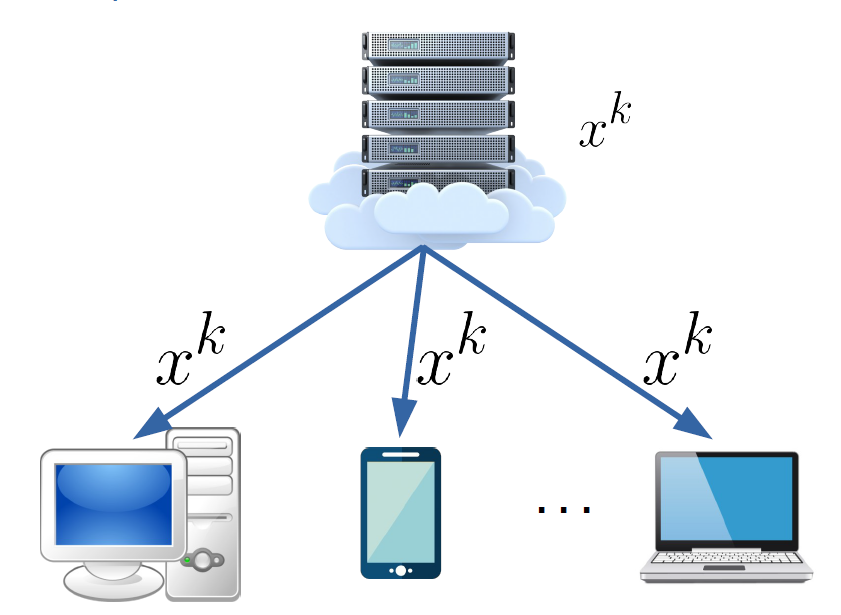
\includegraphics[width=0.4\linewidth]{topology.PNG}
        \end{tabular}
        & \begin{tabular}{l}
            \parbox{0.5\linewidth}{
            Постановка задачи: 
            $$
            \min_{x \in \mathbb{R}^n}\left\{f(x)=\frac{1}{d} \sum_{i=1}^d f_i(x)\right\},
            $$
            Стандартный вид функции на каждом из узлов:
            $$
            f_i(x) = \frac{1}{m} \sum_{j=1}^m f_{ij}(x) \text{ или }
            $$
            $$
            f_i(x) = \mathbb{E}{\left[f_{\phi_i}(x)\right]}.
            $$
            Предположения:
            $$
            f_1, \; f_2 \ldots, \;f_d\; - L\text{-гладкие и выпуклые.}
            $$
            }
        \end{tabular}\\
    \end{tabular}
\end{frame}

\begin{frame}{[1] Задача распределенной минимизации.}
    Основные подходы:
    \begin{itemize}
        \item Изменение топологии
        \item Федерализация
        \item Компрессия
    \end{itemize}

    Используемые функции компрессии:
    \begin{enumerate}
        \item $TopK()$ --- $k$ компонентов,
        \item $RandK()$ --- $k$ случайных компонентов,
        \item $l2-quant()$ --- выделение некоторого вероятностного подпространства. 
    \end{enumerate}

    Предложенный в работе метод:
    $$
    \begin{aligned} 
        x^{k+1} &=x^k-\frac{1}{d} \sum_{i=1}^d v_i^k, \\ 
        e_i^{k+1} &=e_i^k + \gamma g_i^k - v_i^k, \\
        v_i^k &= C(e_i^k + \gamma g_i^k) \quad i=1,2, \ldots, d.
    \end{aligned}
    $$
\end{frame}


\begin{frame}{[1] Задача распределенной минимизации.}
    Экспериментально рассматриваемая задача:
    $$
    \min_{x \in \mathbb{R}^n}\left\{ f(x) = \frac{1}{N} \sum_{i=1}^N \log \left(1+\exp \left(- y_i \cdot(A x)_i\right)\right) + \frac{\mu}{2}\|x\|^2 \right\},
    $$
    \begin{figure}
        \begin{center}
          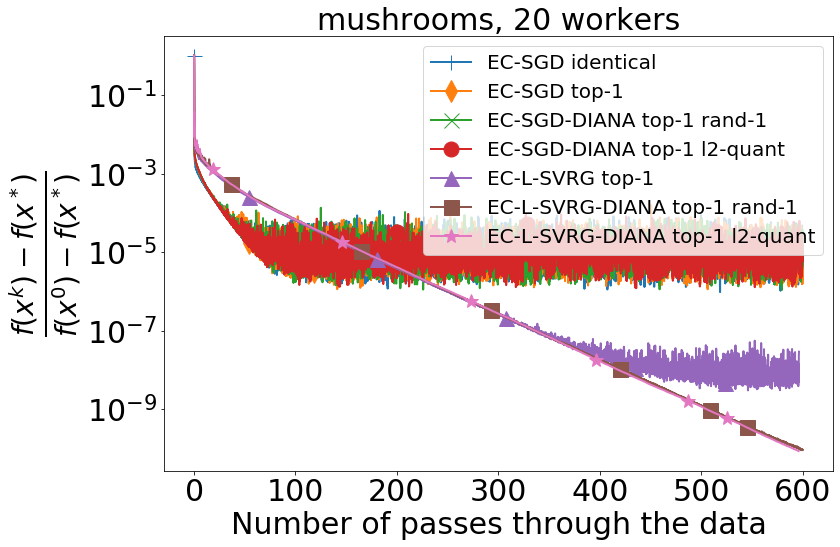
\includegraphics[width=0.8\linewidth]{mushrooms_20.png}
        \end{center}
    \end{figure}
    
\end{frame}

\begin{frame}{[1] Минимизация силового поля.}
    \begin{figure}
    \begin{center}
        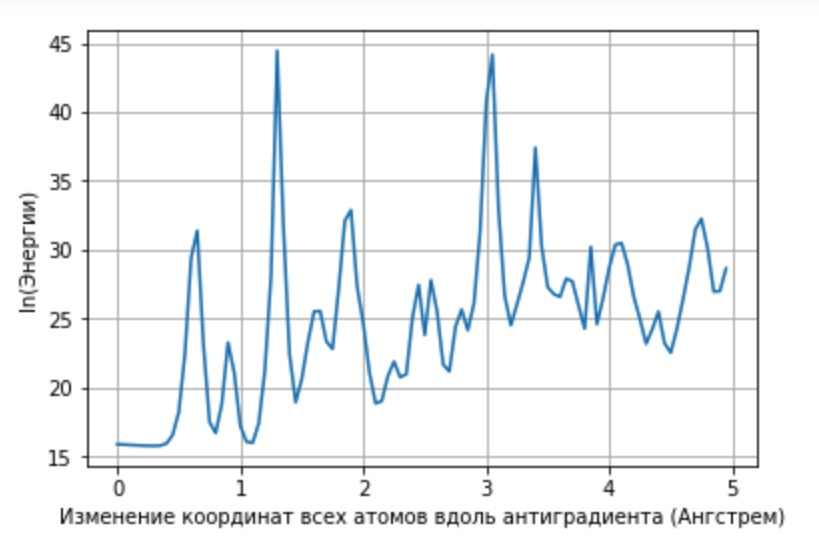
\includegraphics[width=0.85\linewidth]{1DSearch.jpg}
    \end{center}
    \end{figure}
    \begin{table}[h]
    \centering
    \resizebox{\textwidth}{!}{
        \begin{tabular}{|c|c|c|}
            \hline
            \fontsize{12pt}{12pt}\selectfont {\bfseries Показатели} & {\bfseries <<Шевеление>> атома} & {\bfseries Адаптивный градиентный спуск} \\
            \hline
            \fontsize{12pt}{12pt}\selectfont Время 1 итерации, секунды    & 1.2075 & 122.9814 \\
            \hline
            \fontsize{12pt}{12pt}\selectfont Энергия 1 итерации, кДж/моль & 0.0225 & 2.7081 \\
            \hline
            \fontsize{12pt}{12pt}\selectfont $\sim\Delta$Энергии к 300 минуте, кДж/моль & $- 347$ & $- 413$ \\
            \hline
        \end{tabular}
    }
    \end{table}
\end{frame}


\begin{frame}{[2] Оптимальная оценка в негладком случае.}
    В работе \href{https://arxiv.org/abs/1212.2002}{[Lacoste-Julien et al., 2012]} был предложен \textbf{оптимальный} субградиентый метод для:
    \begin{itemize}
        \item задач \textbf{сильно выпуклой} минимизации
        \item в предположении \textbf{липшицевости} целевого функционала
    \end{itemize}
    Задача: $$\min_{x \in Q} f(x)$$
    Метод: $$ x_{k+1} = {Proj}_{Q}(x_k - h_k \nabla f(x_k) ), \; \; где h_k = \frac{2}{\mu (k+1)} $$
\end{frame}


\begin{frame}{[2] Оптимальная оценка в негладком случае.}
    Оценка скорости сходимости: 
    $$
    \label{eq:1} f(\widehat{x}) - f(x_*) \leq \frac{2 M^{2}}{\mu (N+1)} \; \forall x \in Q,
    $$
    
    где $$\widehat{x} = \sum_{k=1}^{N} \frac{2 k}{N (N+1)} \; x_k,  \;\;\;\;\;\; \norm{\nabla f(x)}_{2} \leq M \; \forall x \in Q,$$
    $N$ --- количество итераций, \\
    $\mu$ --- константа сильной выпуклости $f(x)$ 
    
    \vspace{\baselineskip}
    Зеркальный спуск в общем случае:
    $$
    x_{k+1} := \argmin_{x \in Q} \{ h_k \langle \nabla f(x_k), x\rangle + V(x, x_k)\} 
    $$
\end{frame}

\begin{frame}{[2] Необходимые определения.}
    \begin{block}{[Определение] Относительная Липшицевость  \href{https://arxiv.org/pdf/1710.04718.pdf}{[Lu, 2018]}}
        $$
        \langle \nabla f(x), x - y \rangle \leq M\sqrt{2 V(y, x)} \;\;\; \forall x, y \in Q
        $$
    \end{block}

    \begin{exampleblock}{Пример. Функция относительно липшицева, но не липшицева.} 
        Пусть $f(x) := x^2$ для $x \in \mathbb{R}$. Производная $f$ неограничена на $\mathbb{R}$, она не является липшицевой на всей прямой. Введем $d$ как $d(x) := 2x^4$
        Тогда
        $$ V(y, x) = 2y^4 - 2x^4 - 8x^3 (y-x) = \frac{1}{2}(x^2 - y^2) + x^2 (x - y)^2 \geq x^2 (x - y)^2 $$
        Значит, $ (f'(x) (x - y))^2 = 4x^2 (x - y)^2 \leq 2 \cdot 2 V(y,x)$ \\
        \vspace{\baselineskip}
        \centering{ Следовательно $f$ --- $\sqrt{2}$-относительно липшицева.}
    \end{exampleblock}
\end{frame}


\begin{frame}{[2] Необходимые определения.}
    \begin{block}{[Определение] Относительная сильная выпуклость \href{https://arxiv.org/pdf/1610.05708.pdf}{[Lu et al., 2018]}}
        $$
         f(y) \geq f(x) + \langle \nabla f(x), y - x \rangle + \mu V(y, x) \;\;\; \forall x, y \in Q
        $$
    \end{block}
    \begin{exampleblock}{Пример. Функция относительно липшицева и относительно сильно выпукла. \href{https://proceedings.neurips.cc/paper/2020/file/b67fb3360ae5597d85a005153451dd4e-Paper.pdf}{[Zhou et al., 2020]}} 
        Пусть $f(x) := \frac{1}{p}\norm{\cdot}^p_2$ для $p \geq 2$ и $ Q = [-\alpha, \alpha], \; \alpha \ge 0$. Заметим, что $\nabla f(x) = \norm{x}_2^{p - 2} x$ и $\nabla^2 f(x) = \norm{x}_2^{p - 2} I + (p-2)\norm{x}_2^{p - 4} x x^{T}$\\
        $f$ --- является относительно липшицевой с $M = 1$ и $d := \frac{1}{2p}\norm{\cdot}_2^{2p}$\\
        $f$ --- не является сильно выпуклой, т.к. $\nabla^2 f(x) - \mu I$ не является положительно полуопределенной в окрестности 0, но можно подобрать $\mu$, которое удовлетворяет данному условию.
    \end{exampleblock}
\end{frame}


\begin{frame}{[2] Необходимые определения.}
    \begin{block}{[Определение] Относительная сильная монотонность}
        $$ \mu V(y, x) + \mu V(x, y) \leq \langle g(y) - g(x), y - x \rangle  \forall x, y \in Q,$$
    \end{block}
    \begin{exampleblock}{Пример}
        Рассмотрим $f$ --- $\mu$-относительно сильно выпуклая \\
        $$f(x) - f(y) + \mu V(x, y) \leq \langle \nabla{f(x)}, x - y \rangle  \;\; \forall x, y \in Q, $$
        то
        $$f(y) - f(x) + \mu V(y, x) \leq \langle \nabla{f(y)}, y - x \rangle  \forall x, y \in Q, $$
        После сложения последних неравенств, получаем
        $$\mu V(x, y) + \mu V(y, x)\leq \langle \nabla{f(y)} - \nabla{f(x)}, y - x \rangle \;\; \forall x, y \in Q,$$
    \end{exampleblock}
\end{frame}


\begin{frame}{[2] Мотивация для работы с ВН.}
    \begin{exampleblock}{Пример. Функция Лагранжа}
        Функционалы относительно сильно выпуклы:
        $$
        \left\{\begin{aligned}
            \min_{x \in Q} \widehat{g}(x)\\
             g_1(x){,\:}g_2(x){,\:}...\:g_m(x) \leq 0
        \end{aligned}\right.
        $$
        $$L(x, \lambda) = \min_{x \in Q} \max_{\overrightarrow{\lambda} \in \mathbb{R}_+^n} \widehat{g}(x) + \sum_{p=1}^{m} \lambda_p g_p(x) + \varepsilon \norm{V(x)}_*^2$$
    \end{exampleblock}
    Введем оператор:
    $ g(x) := \Bigg( 
      \begin{aligned}
        f^{'}_{u}(u,v)&&\\
        -f^{'}_{v}(u,v)&&
      \end{aligned}
      \Bigg) $
    и ВН: $\langle g(x), x - y \rangle \leq 0$
\end{frame}


\begin{frame}{[2] Теорема для обобщенного случая.}
    \begin{block}{[Теорема]}
        Пусть $g$ --- $\mu$-относительно сильно монотонный оператор и $M$-относительно ограниченный. Тогда после $N$ итераций алгоритма: 
        $$ x_{k+1} := \argmin_{x \in Q} \{ h_k \langle g(x_k), x\rangle + V(x, x_k)\}, \;\;\; h_k = \frac{2}{\mu (k+1)}$$
        будет верно неравенство:
        \begin{equation}\label{eq:2}
            \max_{x \in Q} \langle g(x), \widehat{x} - x\rangle \leq \frac{2 M^2}{\mu (N+1)}
        \end{equation}
    \end{block}
\end{frame}


\begin{frame}{[2] Уточнение оценки при доп. условиях.}
    \begin{block}{[Следствие]}
         $ \max_{x \in Q} \langle g(x), \widehat{x} - x\rangle \leq \varepsilon$
        после $N = \mathcal{O}(\frac{M^2}{\mu \varepsilon})$
    \end{block}
    \begin{block}{[Замечание]}
        Если $d$ --- 1-сильно выпукла и $\norm{g(x)}_* \leq M$, то оценку \eqref{eq:2} можно уточнить
        \begin{equation}
            \max_{x \in Q} \langle g(x), \widehat{x} - x\rangle \leq \frac{2}{\mu N (N+1)} \sum_{k=1}^{N} \frac{k}{k+1} \norm{g(x_k)}_*^2
        \end{equation}
    \end{block}
\end{frame}

\begin{frame}{[2] Случай седловых задач.}
    При рассмотрении выпукло-вогнутой седловой задачи вида:
    \begin{equation}
    \begin{aligned} 
        f^* = \min_{u \in Q_1} \max_{v \in Q_2} f(u, v),
    \end{aligned}
    \end{equation}
    где $f$ --- относительно сильно выпукла по $u$ и относительно сильно вогнута по $v$.

    Обозначим $x = (u, v)$, и введем оператор 
    $$ 
      g(x) := \Bigg( 
      \begin{aligned}
        f^{'}_{u}(u,v)&&\\
        -f^{'}_{v}(u,v)&&
      \end{aligned}
      \Bigg), 
    $$
    что позволяет доказать аналогичную оценку:
    \begin{equation}
    \begin{aligned}
        \max_{v} f(\widehat{u}, v) - \min_{u} f(u, \widehat{v}) \leq \frac{2M^2}{\mu (N+1)}
    \end{aligned}
    \end{equation}
\end{frame}


\begin{frame}{[2] Адаптивный аналог оптимальной оценки.}
    \begin{block}{[Теорема]}
    Пусть $f$ --- $\mu$-сильно выпуклая функция. Тогда после $N$ итераций алгоритма:
    \begin{equation}\label{orig_2}
        x_{k+1} := Pr_{Q}\{x_k - h_k \nabla f(x_k) \}, \;\; \textit{где} \; h_k = \frac{2}{\mu (k+1)}
    \end{equation}
    будет верно неравенство:
    \begin{equation}\label{adaptive_estimation_f}
        f(\widehat{x}) - f(x_*) \leq \frac{2}{\mu N (N+1)} \sum_{k=1}^{N} \frac{k \|\nabla f(x_k)\|_2^2}{k+1},
    \end{equation}
    где
    $$
        \widehat{x} = \sum_{k=1}^{N} \frac{2 k}{N (N+1)} x_k.
    $$
    \end{block}
\end{frame}


\begin{frame}{[2] Эксперименты. Удаленность от решения.}
    Рассматривается задача о нахождении наименьшего покрывающего шара:
    \begin{gather}\label{sphere_cover_strongly}
        f(x) := \max_{x\in Q}\left\{\|x - a_0\|_2^2, \|x - a_1\|_2^2, ..., \|x - a_m\|_2^2\right\},
    \end{gather}
    \begin{figure}
        \centering
        \includegraphics[width=1\linewidth]{"compare_radius"}
    \end{figure}
\end{frame}


% \begin{frame}{[2] Эксперименты. Неограниченное Q.}
% \begin{columns}
%     \begin{column}{0.55\textwidth}
%     \begin{figure}
%         \centering
%         \includegraphics[width=1\linewidth]{"q_unlim"}
%     \end{figure}
%     \end{column}
        
%     \begin{column}{0.55\textwidth}
%     \begin{figure}
%         \centering
%         \includegraphics[width=1\linewidth]{"q_unlim_raw"}
%     \end{figure}
%     \end{column}
% \end{columns}
% \end{frame}


% \begin{frame}{[3] Сравнение .}
%     \begin{block}{[Определение] Условие острого минимума \href{https://doi.org/10.1016/0041-5553(69)90061-5}{[Polyak, 1969]}}
%         \begin{equation}
%             f(x) - f(x_*) \geq \alpha \min_{x_* \in X_*}{\| x - x_* \|_2} \text{ при } \alpha > 0\;\; \forall x \in Q
%         \end{equation}
%     \end{block}
%     Мотивация для сравнения наверное
% \end{frame}

\begin{frame} {[3] Сильная выпуклость и острый минимум.}
    \begin{figure}[H]
        \minipage{0.49\textwidth}
        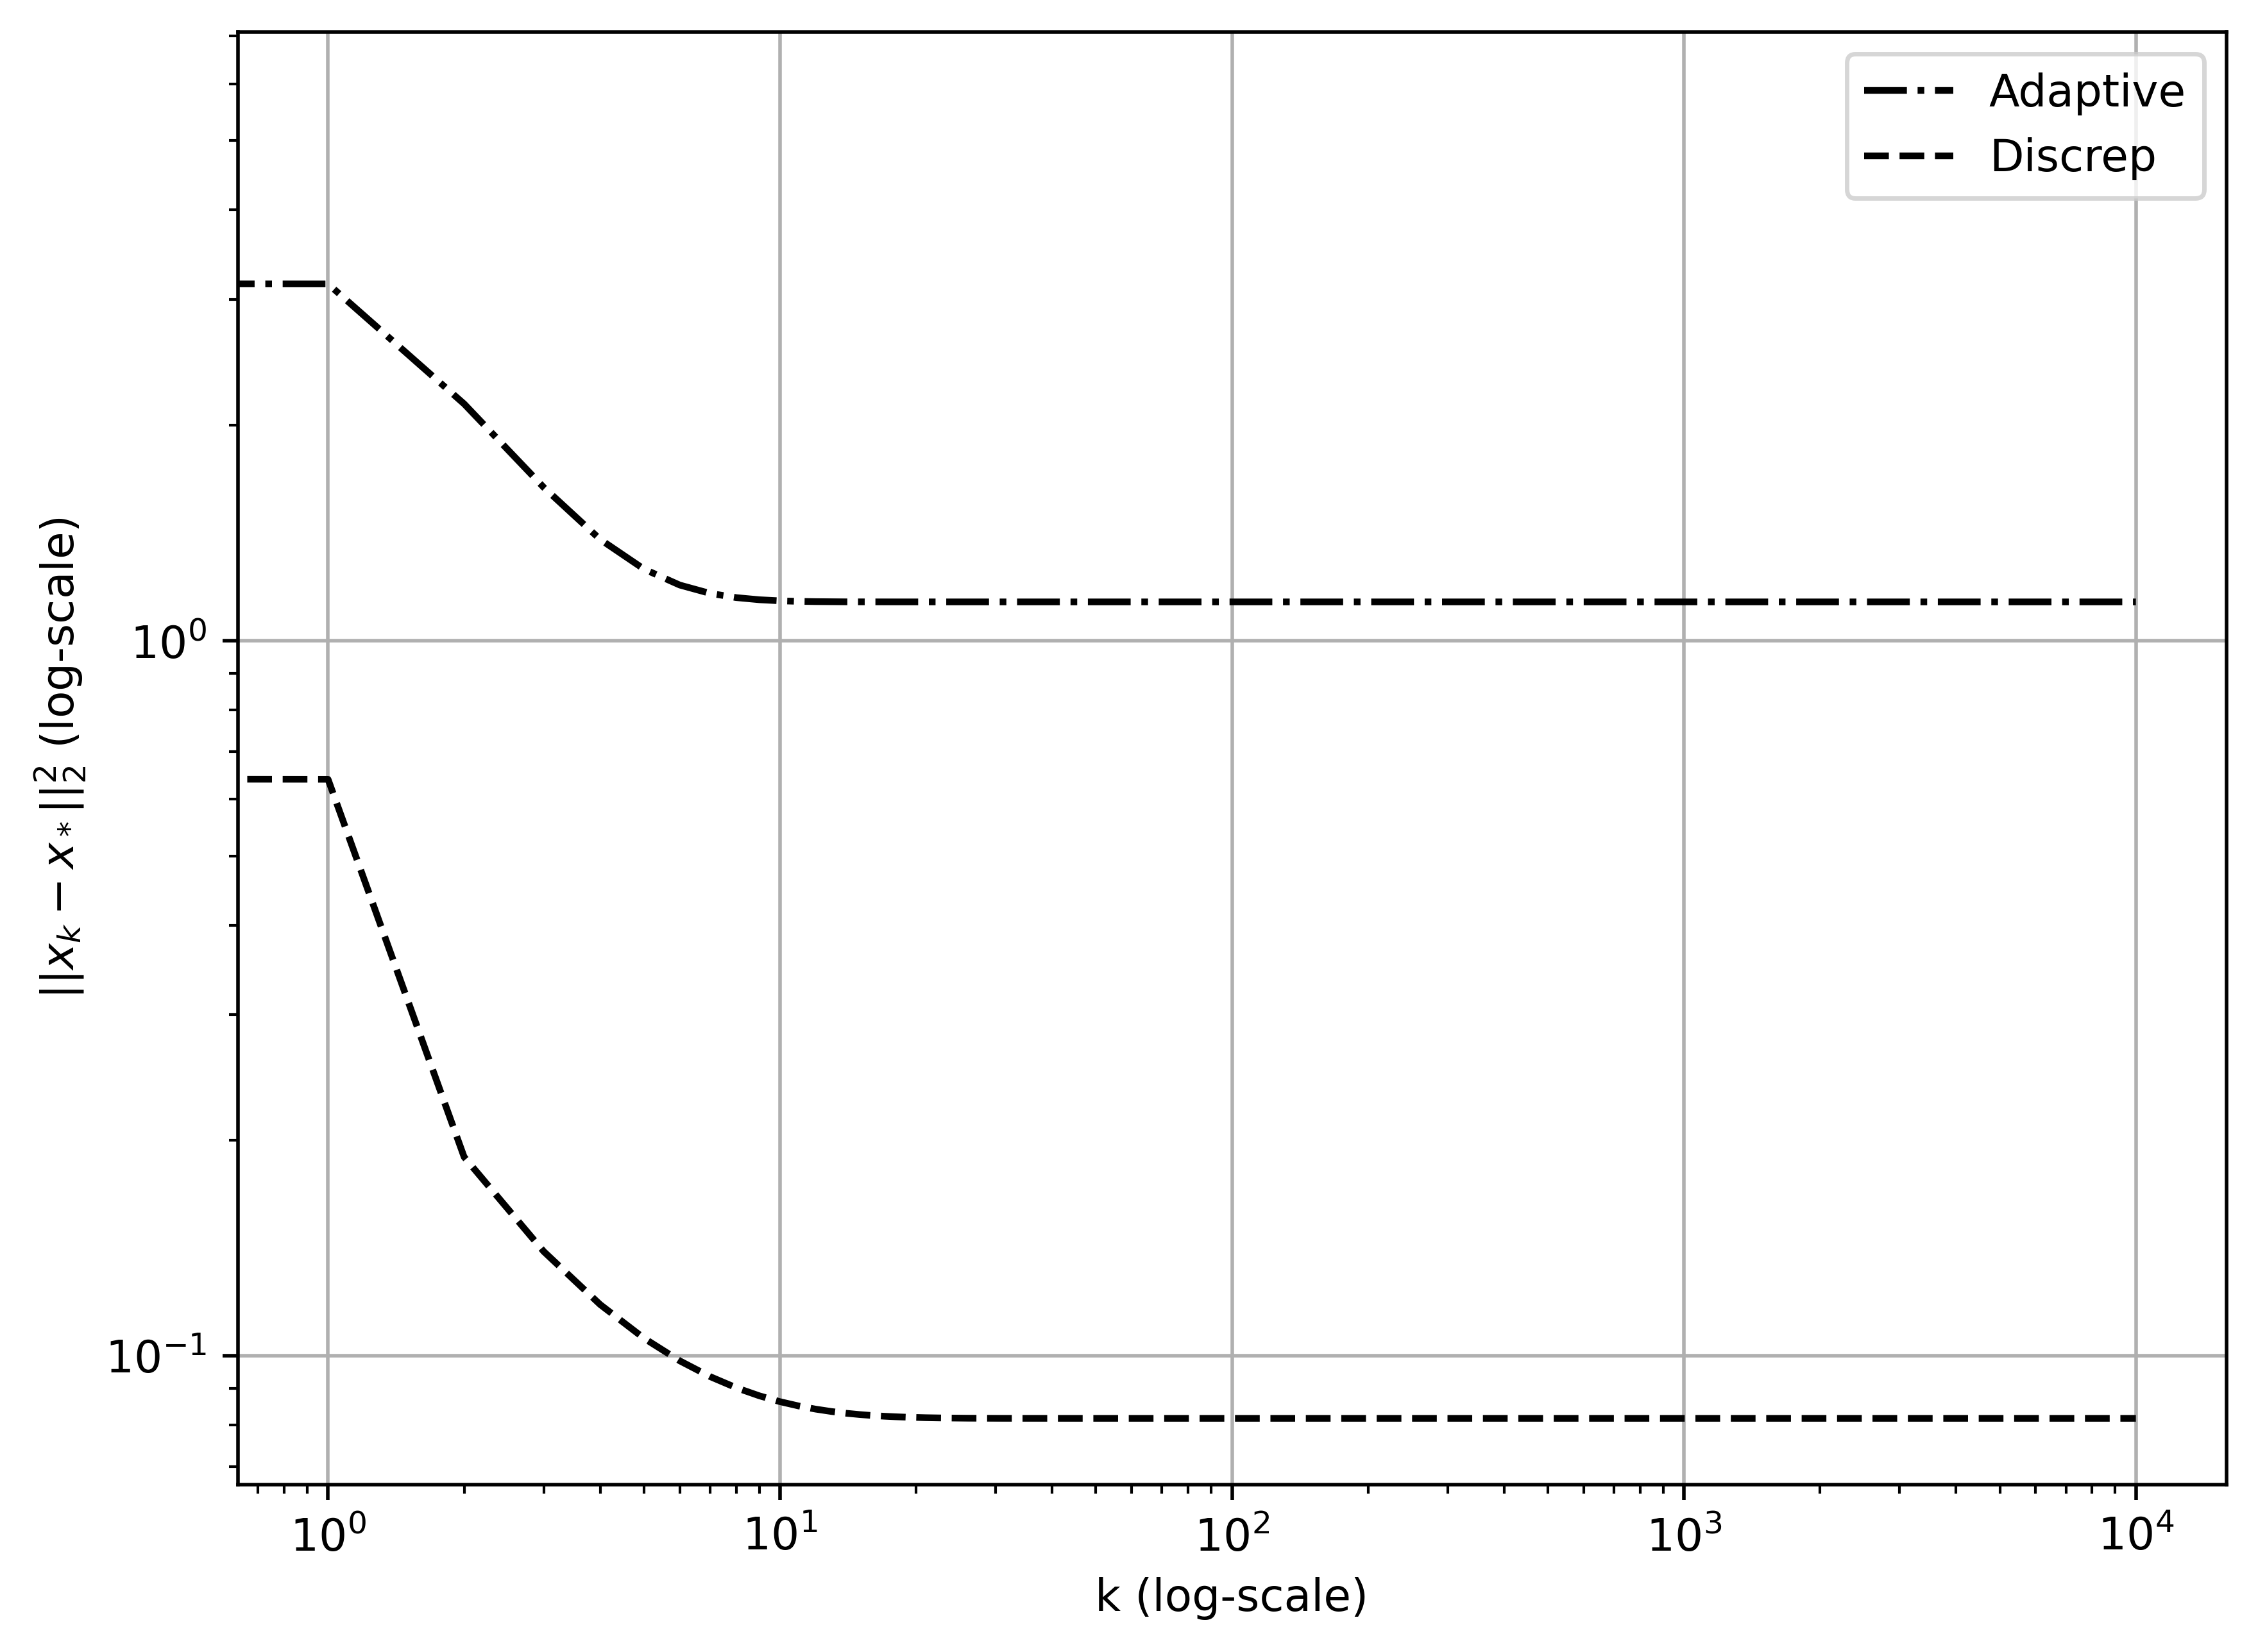
\includegraphics[width=\linewidth]{sharp_convex_x.png}
        \endminipage\hfill
        \minipage{0.49\textwidth}
        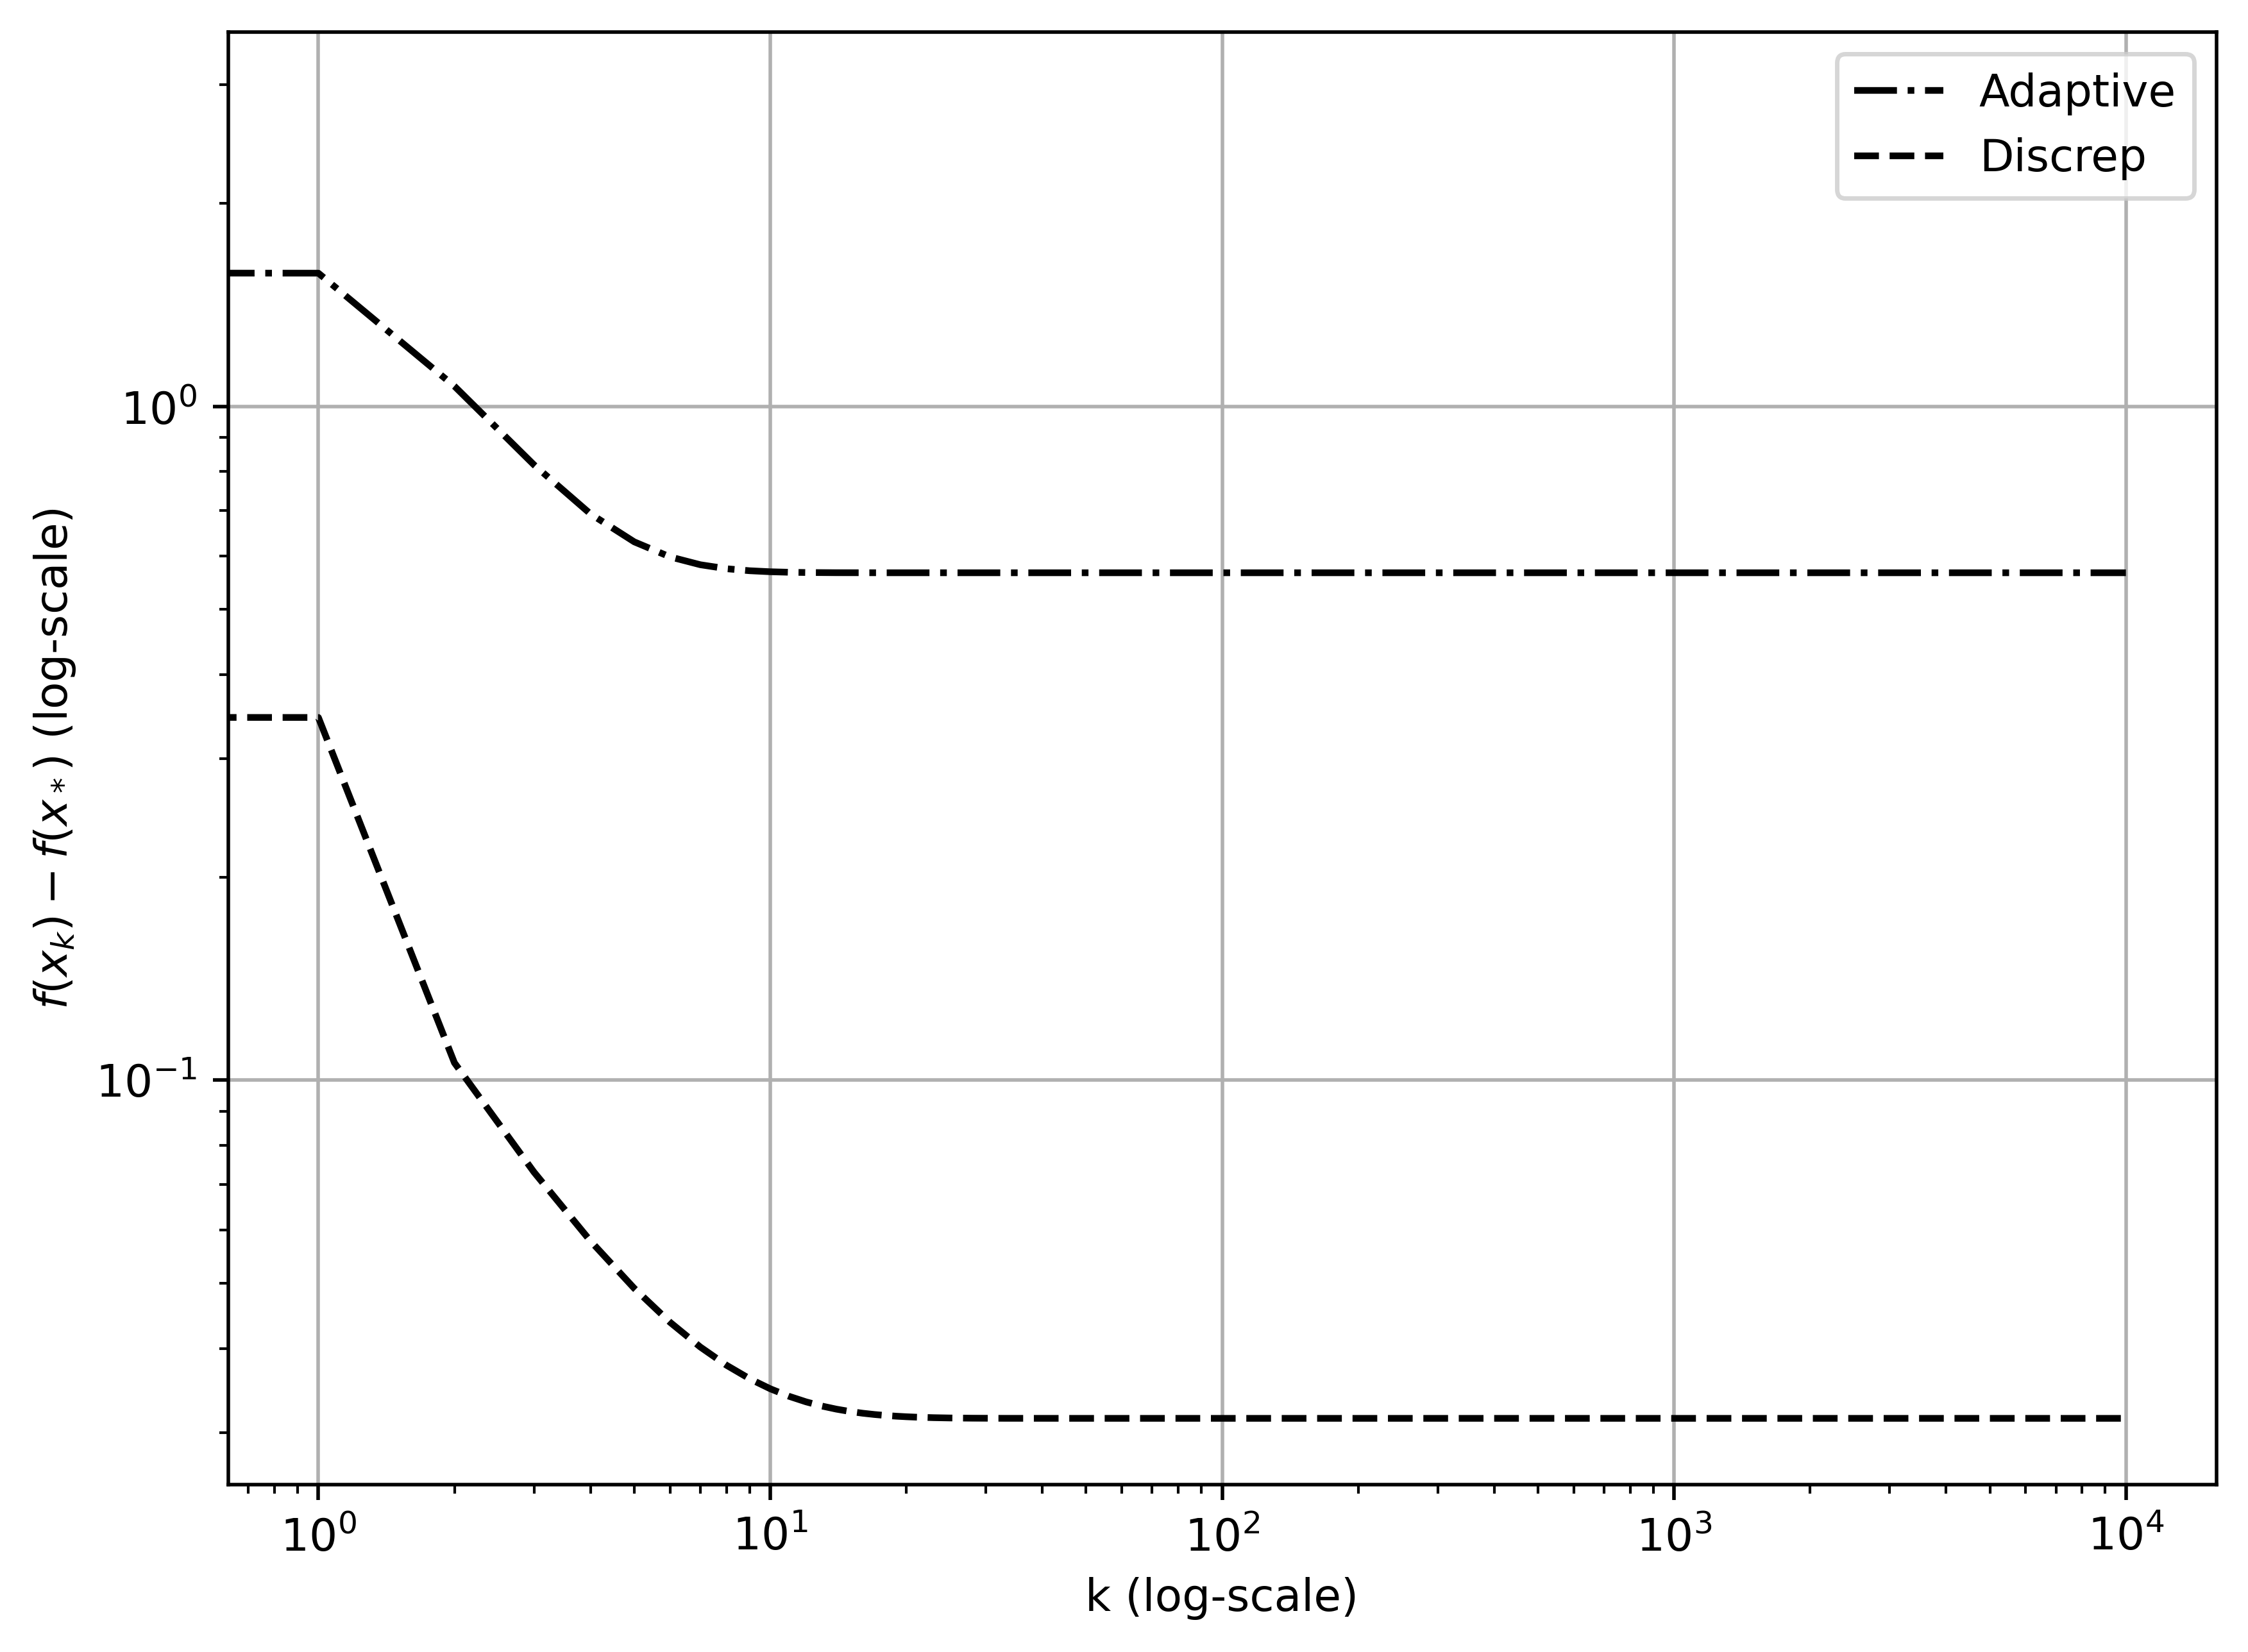
\includegraphics[width=\linewidth]{sharp_convex_f.png}
        \endminipage\hfill
        \label{res_sharp_convex}
    \end{figure}
    
    \begin{figure}[H]
        \minipage{0.49\textwidth}
        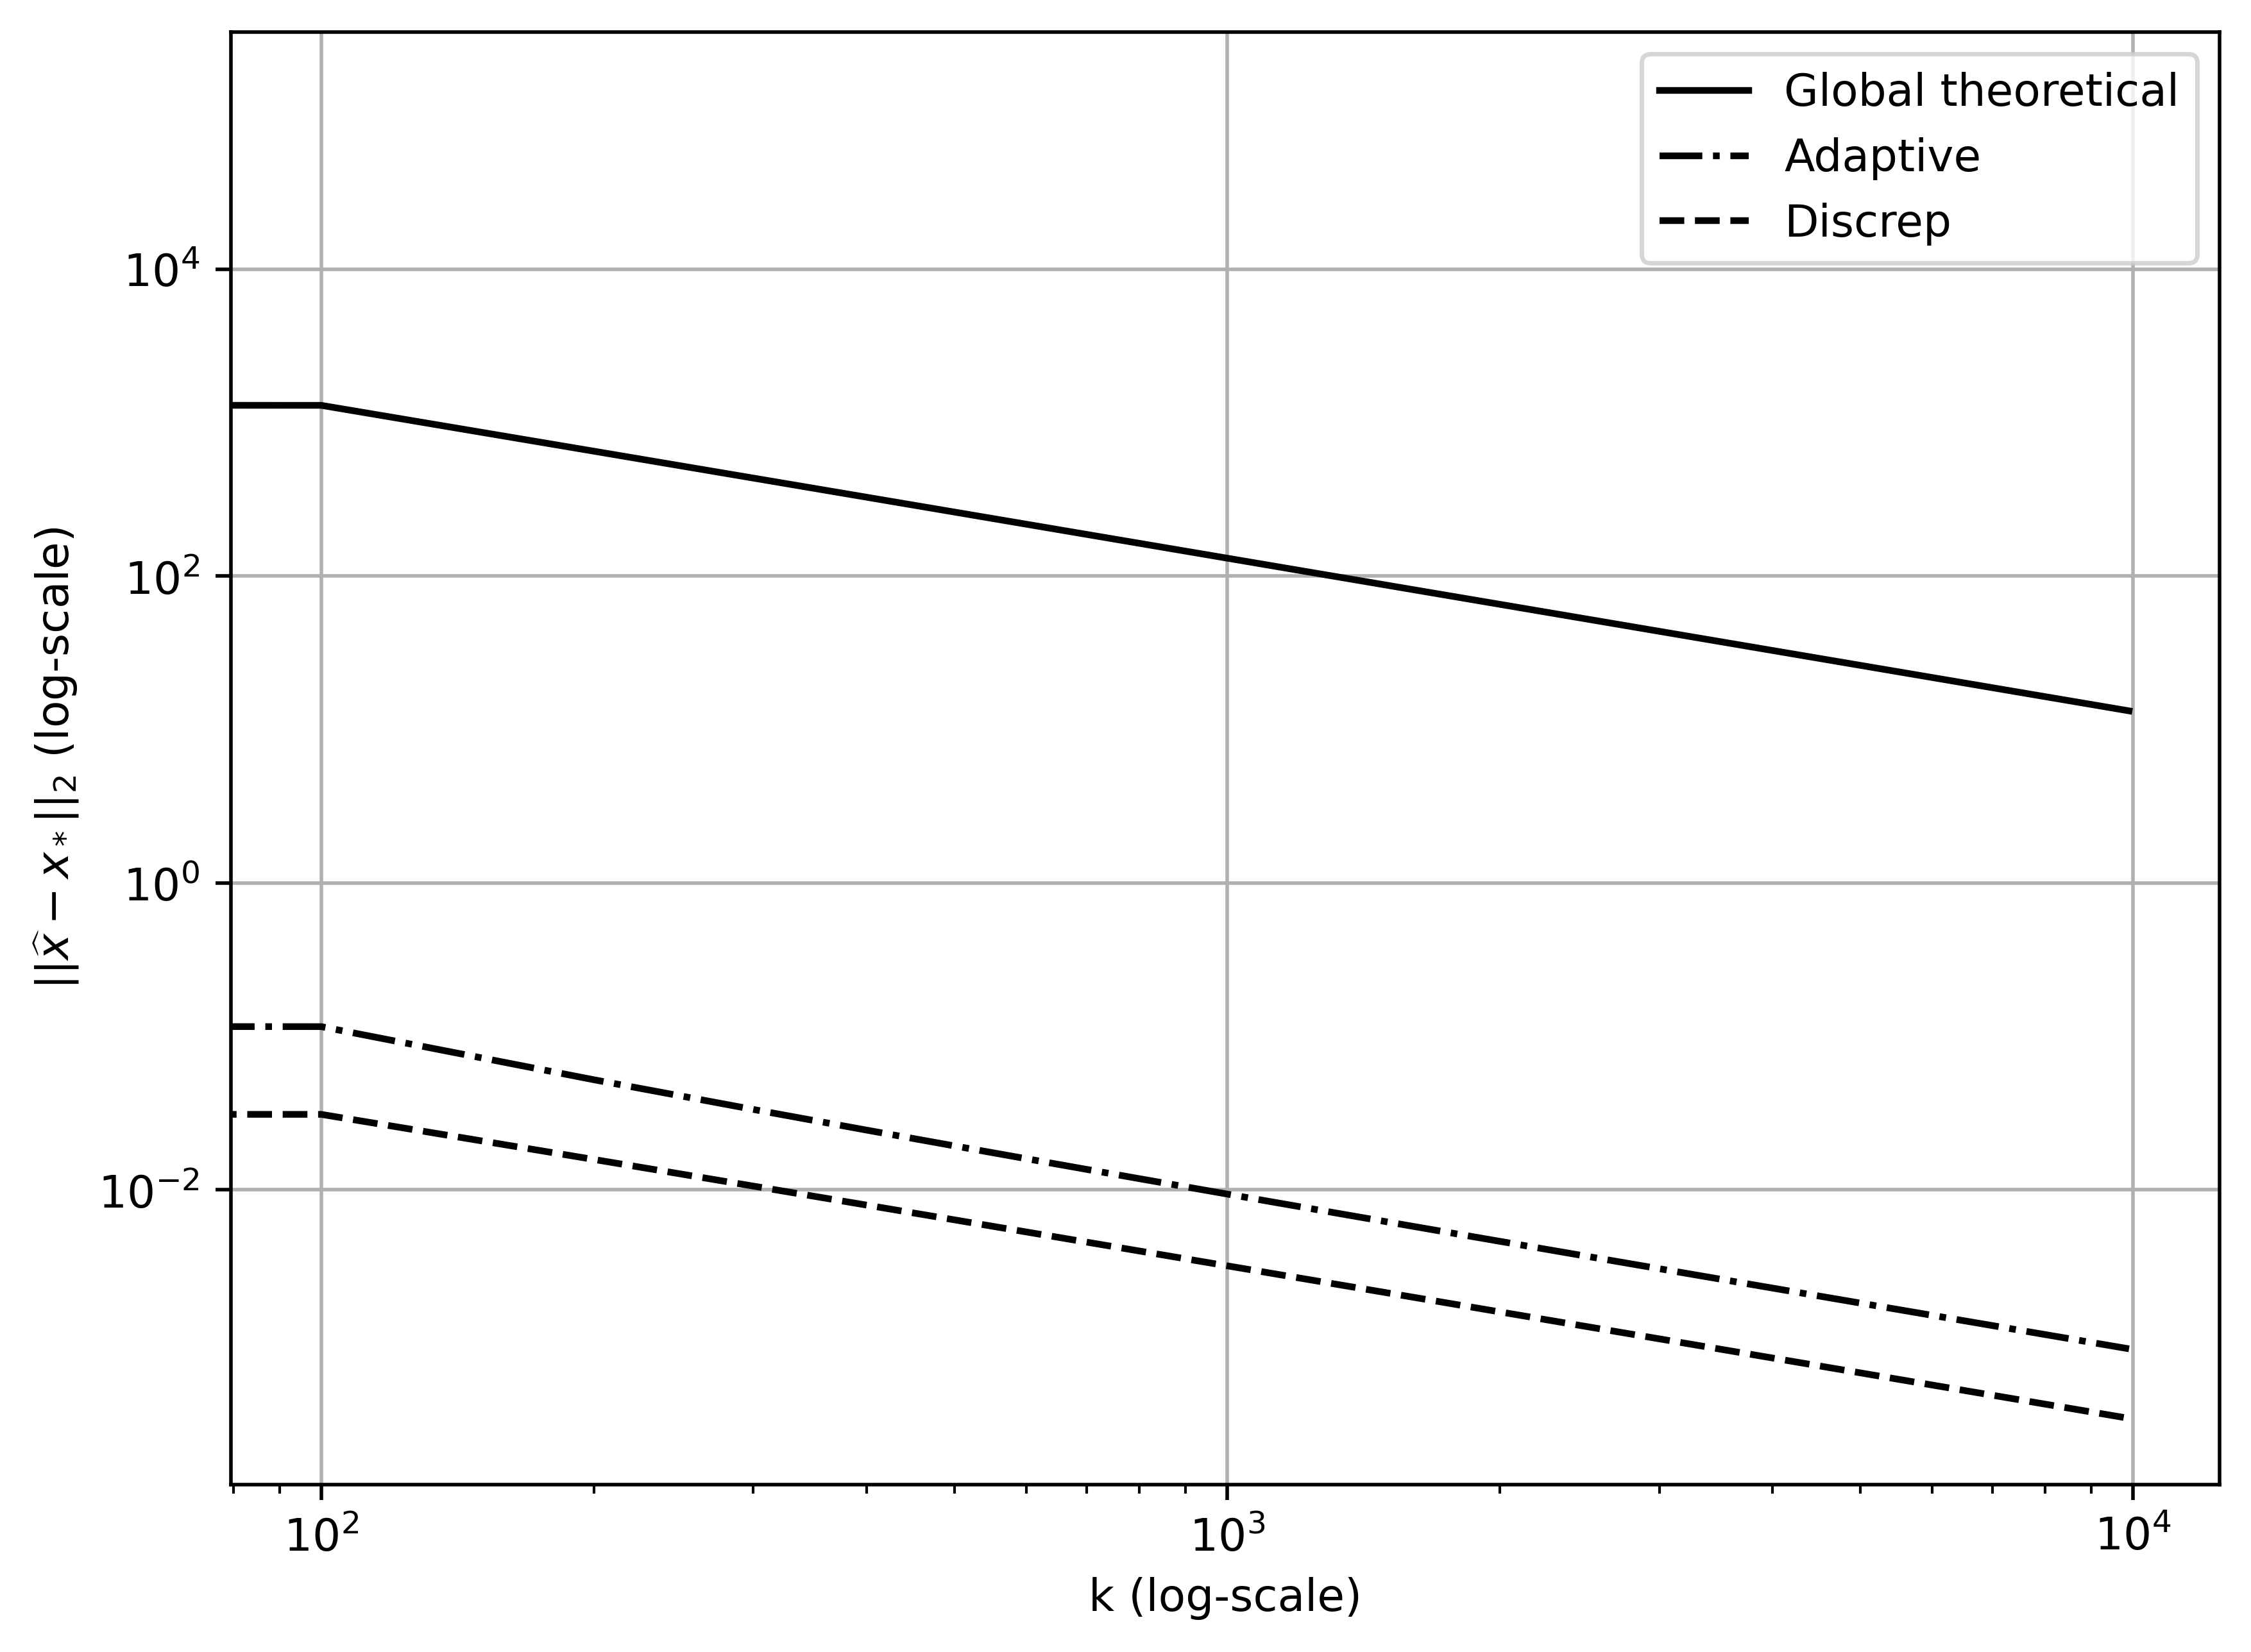
\includegraphics[width=\linewidth]{strong_convex_small_rad_x.png}
        \endminipage\hfill
        \minipage{0.49\textwidth}
        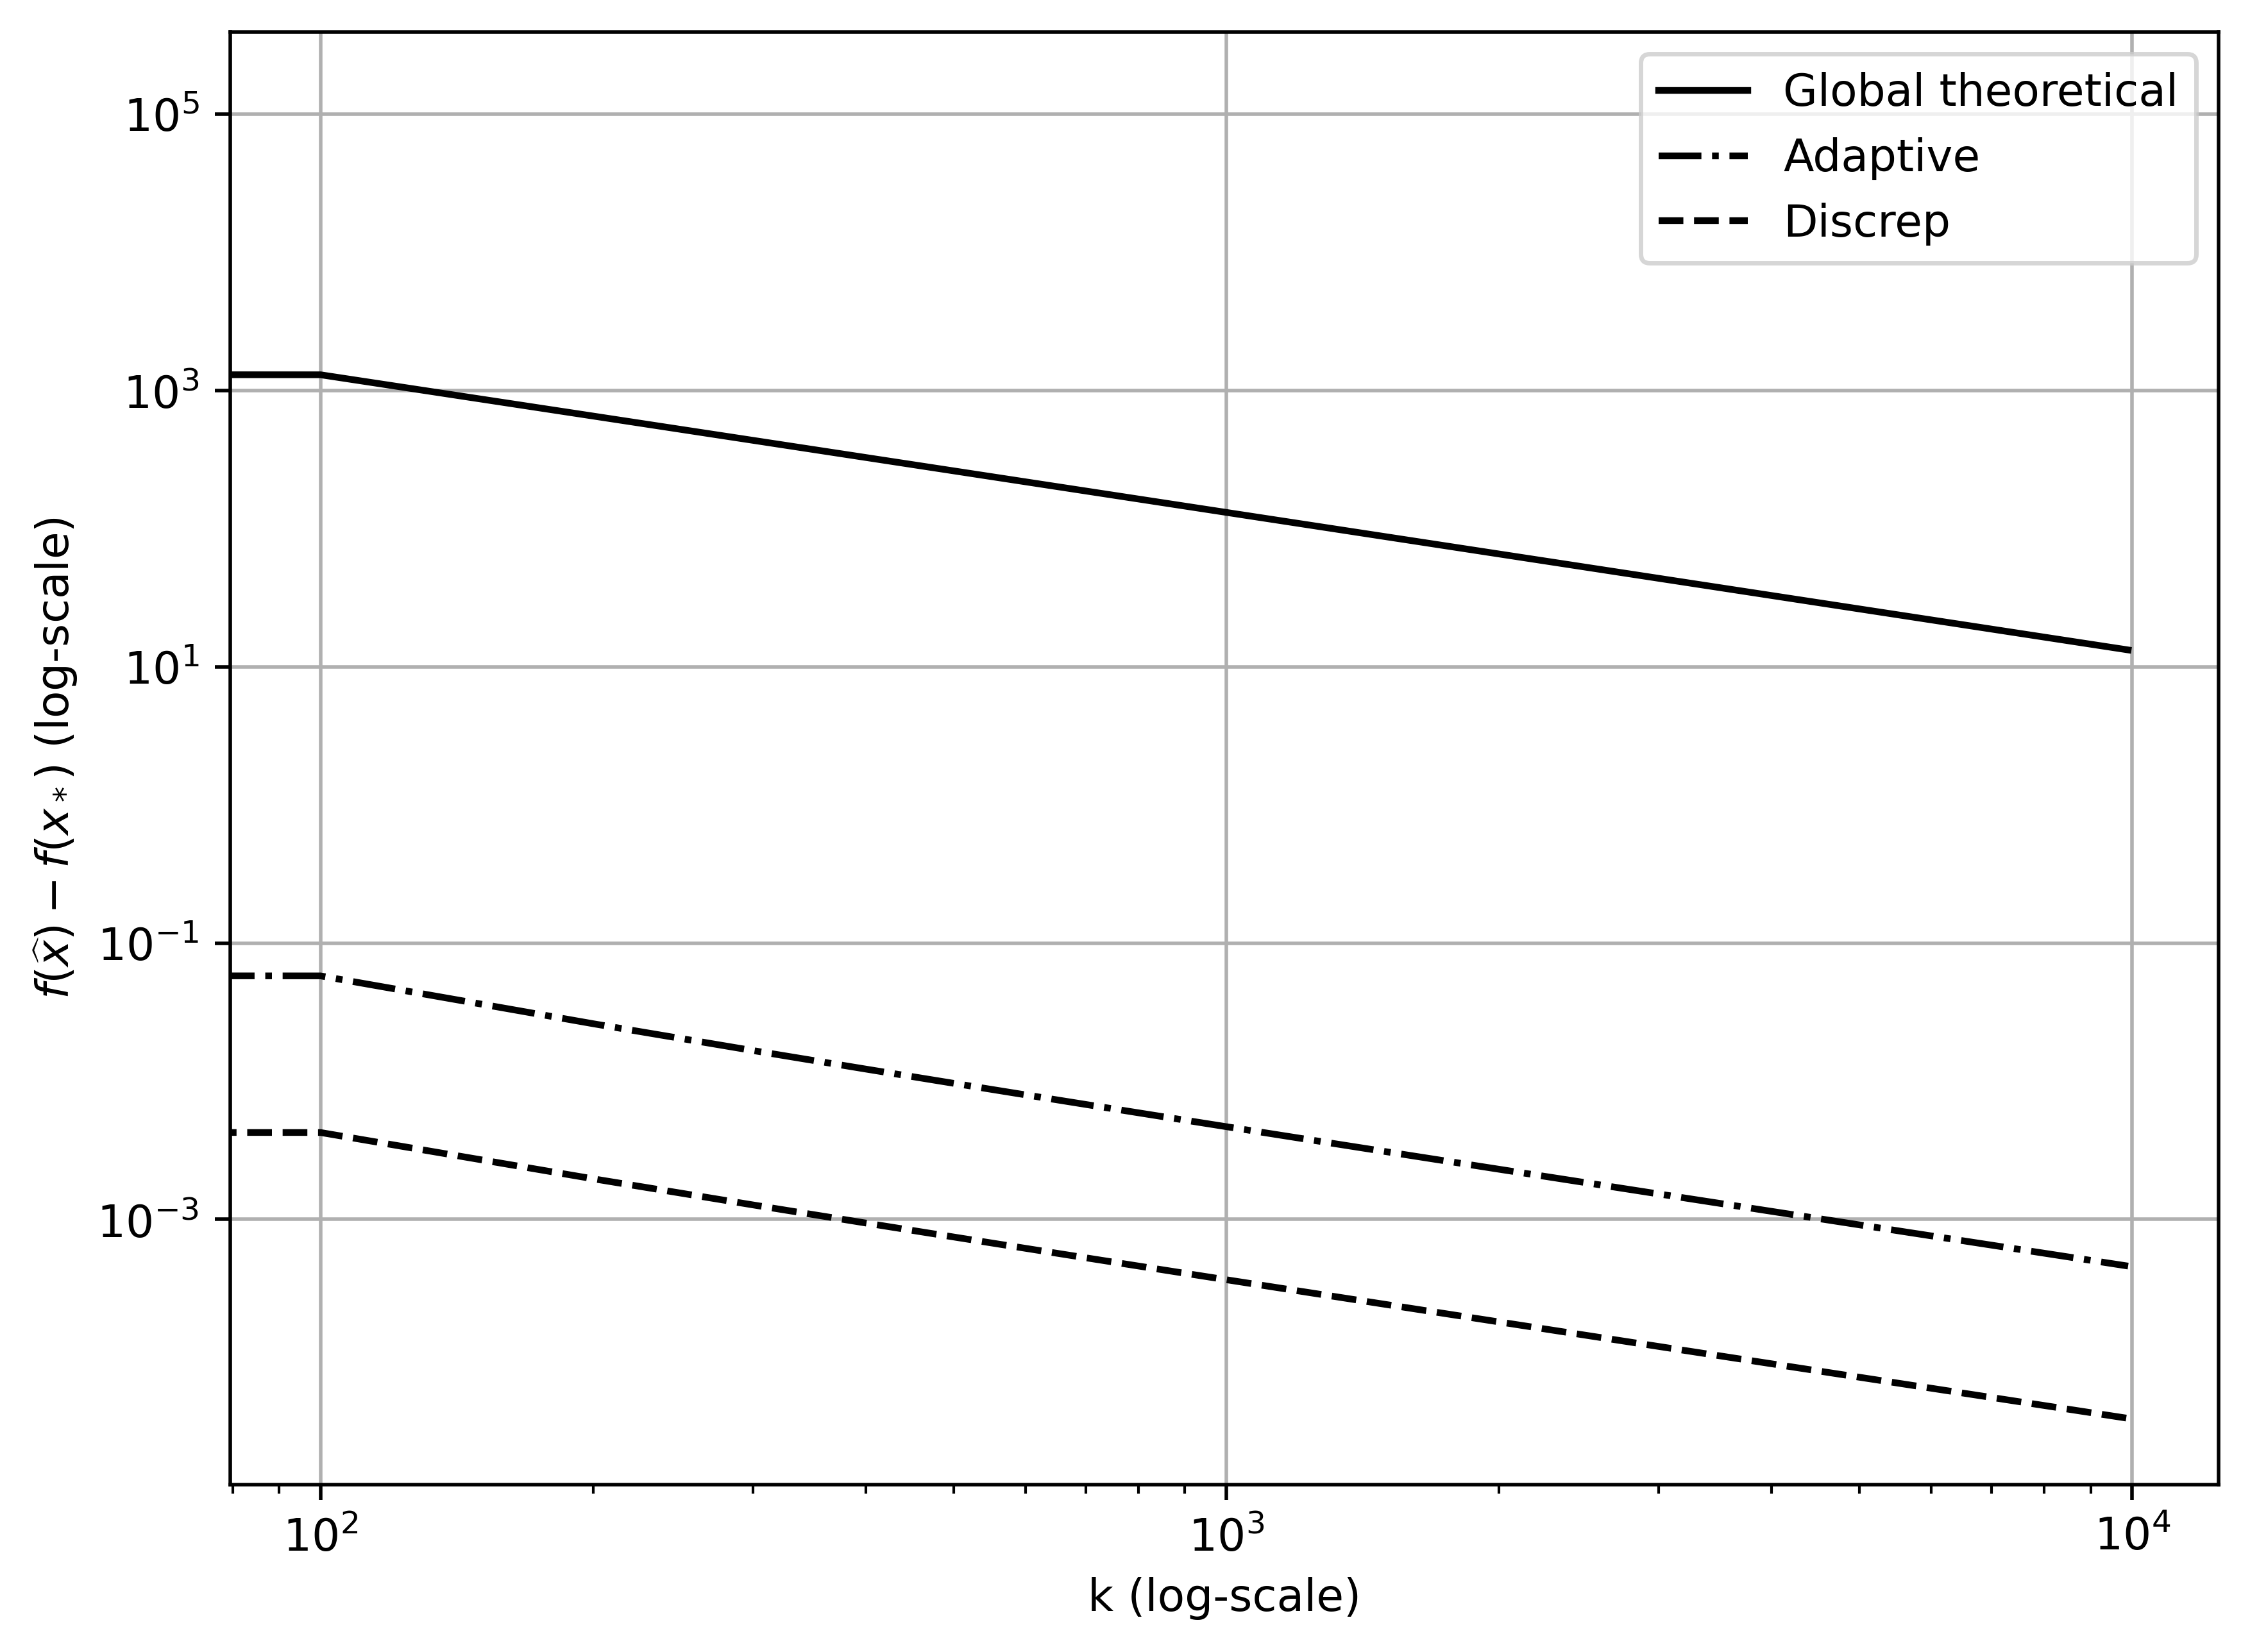
\includegraphics[width=\linewidth]{strong_convex_small_rad_f.png}
        \endminipage\hfill
        \label{res_strong_convex}
    \end{figure}
\end{frame}

\begin{frame}{[3] Обобщение понятия острого минимума.}
    \begin{block}{[Определение] Условие острого минимума \href{https://doi.org/10.1016/0041-5553(69)90061-5}{[Polyak, 1969]}}
        \begin{equation}
            f(x) - f(x_*) \geq \alpha \min_{x_* \in X_*}{\| x - x_* \|_2} \text{ при } \alpha > 0\;\; \forall x \in Q
        \end{equation}
    \end{block}
    \begin{block}{[Определение] Условие относительного $\gamma$-роста}
        Будем говорить, что $f$ удовлетворяет условию относительного $\gamma$-роста, если для всякого $x \in Q$ верно неравенство:
        \begin{equation} \label{gamma-growth}
            f(x) - f(x_*) \geq \mu_{\gamma}\left(\min_{x_* \in X_*}{V(x_*,x)}\right)^{\gamma/2},
        \end{equation}
        где $X_*$ --- множество точных решений задачи минимизации $f$. 
    \end{block}
\end{frame}


\begin{frame} {[3] Алгоритм рестартов}
Введем следующее обозначение
\[
    x_{min}^j  := \argmin_{0\leq k \leq N} f(x_k) \;\;\; \text{на} \;\; j\text{-м рестарте}.
\]
\begin{algorithm}[H]
    \label{alg:rest_gamma}
    %\caption{Рестарты зеркального спуска при условии относительного $\gamma$-роста.}
    \setstretch{1.25}
    \DontPrintSemicolon
    \KwData{$\varepsilon > 0$}
    \KwResult{$x_p$}
    $p \gets 0$\;
    \While{$p < \frac{1}{\gamma} \log_2{\left[\frac{\mu_{\gamma}^2}{\varepsilon^2} \left(\min\limits_{x_* \in X_*}{V(x_*, x_0^0)}\right)^{\gamma} \right]}$ \;}{
        $x_{p}$ --- результат зеркального спуска с параметром $N_{p} = \ceil*{\frac{2^{\gamma+1} M^2}{\mu_{\gamma}^2 2^{p(1 - \gamma)}} \left(\min\limits_{x_* \in X_*}{V(x_*, x_0)}\right)^{1 - \gamma}}$\;
        $x_0 = x_{min}^p$\;
        $p=p+1$\;
    }
\end{algorithm}
\end{frame}


\begin{frame} {[3] Оценки для алгоритма рестартов.}
\begin{block}{[Теорема]} \label{simple_restart}
    Пусть $f$ удовлетворяет условию относительного $\gamma$-роста \eqref{gamma-growth} и также является относительно $M$-липшицевой на $Q$. В таком случае алгоритм \ref{alg:rest_gamma} после 
    \begin{equation}
    \begin{aligned}
       N =\mathcal{O}\left(\frac{4 M^2}{\mu_{\gamma}^2} \log_2{\left[\frac{\mu_{\gamma}^2}{\varepsilon^2} \left(\min\limits_{x_* \in X_*}{V(x_*, x_0^0)}\right) \right]}\right) \text{ при } \gamma = 1, \\
       N = \mathcal{O}\left(\frac{2^{\gamma + 1} M^2}{2^{(\gamma - 1)} - 1}\left[\frac{1}{\mu_{\gamma}^{\frac{2}{\gamma}}} \varepsilon^{\frac{2(1 - \gamma)}{\gamma}}  - \frac{1}{\mu_{\gamma}^2 \left(\min\limits_{x_* \in X_*}{V(x_*, x_0^0)}\right)^{(\gamma - 1)}} \right]\right) \\
       \text{ при } \gamma > 1,
    \end{aligned}
    \end{equation}
    обращений к субградиенту $f$ будет справедливо неравенство
    \begin{equation}
        f(x_{min}^{p-1}) - f(x_*) \leq \varepsilon.
    \end{equation}
\end{block}
\end{frame}

\begin{frame} {[3] Алгоритм рестартов с критерием остановки.}
\begin{algorithm}[H]
    %\caption{Рестарты зеркального спуска при условии $\gamma$-роста с критерием остановки.}
    \label{alg:rest_criteria}
    \setstretch{1.25}
    \DontPrintSemicolon
    \KwData{$\varepsilon > 0$}
    \KwResult{$x_p$}
    $p \gets 0$\;
    $\Theta_0^2 \geq \min\limits_{x_* \in X_*}{V(x_*,x_0)}$\;
    \While{$p < \log_2{\left[\left(\frac{\mu_{\gamma}}{\varepsilon}\right)^{\frac{2}{\gamma}} \Theta_0^2\right]}$\;}{
        $x_{p}$ --- результат зеркального спуска с критерием остановки $\sum_{k=0}^{N_p} \frac{1}{\norm{\nabla f(x_k) }_*^2} \geq \frac{ 2^{(p \gamma - p  + 1)}}{\mu_{\gamma}^2 \Theta_0^{2\gamma - 2} }$\;
        $x_0 = x_{min}^p$\;
        $p=p+1$\;
    }
\end{algorithm}
\end{frame}


\begin{frame} {[3] Оценки для алгоритма рестартов с критерием остановки.}
\begin{block}{[Теорема]} \label{simple_restart}
    Пусть $f$ выпукла и удовлетворяет условию относительного $\gamma$-роста \eqref{gamma-growth} с 1-сильно выпуклой прокс-структурой, а также является $M$-липшицевой на $Q$. В таком случае после работы алгоритма \ref{alg:rest_criteria} будет справедливо неравенство
    \begin{equation}
        f(x_{min}^{p-1}) - f(x_*) \leq \varepsilon.
    \end{equation}
    Для этого потребуется не более чем
    \begin{equation}
       N = \mathcal{O} \left( \frac{4 M^2}{\mu_{\gamma}^2} \log_2{\left[\frac{\mu_{\gamma}^2 \Theta_0^2}{\varepsilon^2} \right]} \right) \text{ при } \gamma = 1,
    \end{equation}
    \begin{equation}
       N = \mathcal{O}\left( \frac{2^{(\gamma + 1)} M^2 }{2^{(\gamma - 1)} - 1}\left[ \frac{1}{\mu_{\gamma}^{\frac{2}{\gamma}}} \varepsilon^{\frac{2}{\gamma} - 2} - \frac{1}{\mu_{\gamma}^2 \Theta_0^{2(\gamma - 1)}} \right] \right) \text{ при } \gamma > 1.
    \end{equation}
\end{block}
\end{frame}

